\documentclass{article}
\usepackage{geometry}
\usepackage{pgfplots}
\usepackage{graphicx}
\usepackage{multirow}
\usepackage{fancyvrb}
\pgfplotsset{compat=1.9}

\geometry{a4paper, margin=1in}
\renewcommand{\thesection}{\Alph{section}.}

\begin{document}

{\Large Lab 04b Program 5}
\vspace{0.25in}

\noindent
By submitting this assignment, I agree to the following: \\
 ``Aggies do not lie, cheat, or steal, or tolerate those who do'' \\
 ``I have not given or received any unauthorized aid on this assignment'' \\

\noindent
Name:        Rushil Udani \\*
Section:     219 \\*
Assignment:  04b Program 5 \\*
Date:        15 09 2020 \\*

\hrulefill

\section*{Given information}

\textbf{Goal: Prompt the user for a strain value, then calculate and report the \textit{stress} value and the \textit{region} the value falls within.}

\begin{figure}[h]
	\begin{minipage}[c]{0.45\linewidth}
		\centering
		\includegraphics[width=4in]{streb.png}
	\end{minipage}
	\hfill
	\begin{minipage}[c]{0.45\linewidth}
		\centering
		\begin{tabular}{l||l}
			Section & Points \\ \hline
			Linear Elastic & O - A \\
			\textit{Ignored} & A - B \\
			Plastic & B - C \\
			Strain Hardening & C - D \\
			Necking & D - E \\
		\end{tabular}
	\end{minipage}
\end{figure}

\section{Linear Model}

\begin{figure}[h]
\begin{minipage}[c]{0.45\linewidth}
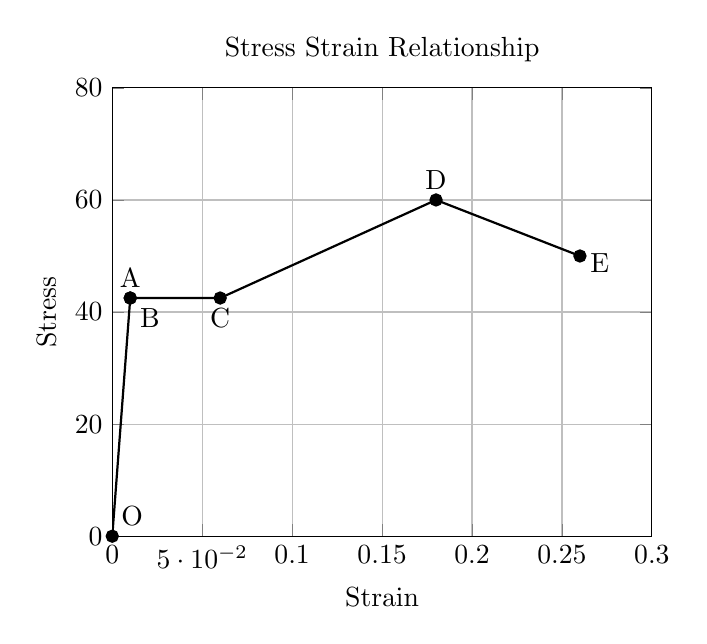
\begin{tikzpicture}
	\begin{axis}[
		title = {Stress Strain Relationship},
		xlabel = {Strain}, ylabel = {Stress},
		xmin = 0, xmax = 0.30,
		xmajorgrids = true,
		ymin = 0, ymax = 80,
		ymajorgrids = true,
		visualization depends on=\thisrow{alignment} \as \alignment,
		nodes near coords,
		point meta=explicit symbolic,
		every node near coord/.style={anchor=\alignment},
		]
		\addplot[
			black,
			thick,
			mark=*,
			] table [meta index=2] {
				x      y     label  alignment
				0      0     O      225
				0.01   42.5  A      270
				0.01   42.5  B      135
				0.06   42.5  C      90
				0.18   60    D      270
				0.26   50    E      160
			};
	\end{axis}
\end{tikzpicture}
\end{minipage}
\hfill
\begin{minipage}[t]{0.35\linewidth}
	\begin{tabular}{l||l|l}
		Point & x & y \\ \hline
		O & 0 & 0 \\
		A & 0.01 & 42.5 \\
		B & 0.01 & 42.5 \\
		C & 0.06 & 42.5 \\
		D & 0.18 & 60 \\
		E & 0.26 & 50 \\
	\end{tabular}
\end{minipage}
\end{figure}

\section{Values and Variables}

\begin{tabular}{p{0.15\textwidth}|p{0.15\textwidth}|p{0.6\textwidth}}
	Name & Type & Description \\ \hline \hline
	\verb/user_strain/ & \verb/float/ & The given strain on the object. \\ \hline
	% The following \Verb is broken to allow a line break to form there. 
	\verb/O/ & \multirow{5}{0.2\linewidth}{\Verb/tuple[float,/ \Verb/float]/} & \multirow{5}{0.6\linewidth}{The value, as \Verb/(strain, stress)/, that this point corresponds to.} \\ \cline{0-0}
	\verb/A/ & & \\ \cline{0-0}
	\verb/B/ & & \\ \cline{0-0}
	\verb/C/ & & \\ \cline{0-0}
	\verb/D/ & & \\ \cline{0-0}
	\verb/E/ & & \\ \hline
	\verb/region/ & \verb/string/ & The name of the region that \verb/user_strain/ is in. \\ \hline
	\verb/strain1/ & \multirow{4}{0.2\linewidth}{\Verb/float/} & \multirow{4}{0.6\linewidth}{The information needed to perform linear interpolation. Should contain the values of the points on either side of \Verb/user\_strain/.} \\ \cline{0-0}
	\verb/strain2/ & & \\ \cline{0-0}
	\verb/stress1/ & & \\ \cline{0-0}
	\verb/stress2/ & & \\ \hline
	\verb/calc_stress/ & \verb/float/ & The predicted stress that we have just computed. \\
\end{tabular}

\section{Procedure}

\begin{enumerate}
	\item Get user input for value of \verb/user_strain/.
	\item Find in what portion of the domain it is.
		\begin{enumerate}
			\item Check if \verb/user_strain/ is below \verb/A[0]/, the strain at point \verb/A/.
			\item If it is, set \verb/O/ to be the left bound (\verb/strain1/ and \verb/stress1/) and \verb/A/ to be the right bound (\verb/strain2/ and \verb/stress2/). Additionally, assign \verb/region/ with the name of this region.
			\item If it is not, repeat with \verb/B/, and then \verb/C/, and so on, using the appropriate points to fill in the \verb/strain/s and \verb/stress/es.
		\end{enumerate}
	\item Calculate an expected stress value.
		\begin{enumerate}
			\item Set up a linear interpolation using \verb/strain1/, \verb/strain2/, \verb/stress1/, and \verb/stress2/.
			\item Calculate a predicted stress using \verb/user_strain/.
		\end{enumerate}
	\item Display the \verb/region/ and \verb/calc_stress/ variables. 
\end{enumerate}

\section{Test Cases}

\begin{tabular}{p{0.1\textwidth}|p{0.1\textwidth}|p{0.1\textwidth}|p{0.1\textwidth}|p{0.5\textwidth}}
	Input & Expected & Region & Type & Notes \\ \hline \hline
	0.005 & 21.25 & O - A & Typical & \multirow{4}{*}{Should be able to interpolate from the given points} \\ \cline{0-3}
	0.03 & 42.5 & B - C & Typical & \\ \cline{0-3}
	0.1 & 4.833 & C - D & Typical & \\ \cline{0-3}
	0.2 & 52.5 & D - E & Typical & \\ \hline
	0 & 0 & O & Edge & This is Point O \\ \hline
	0.01 & 42.5 & A, B & Edge & This is Points A and B \\ \hline
	0.06 & 42.5 & C & Edge & This is Point C \\ \hline
	0.18 & 60 & D & Edge & This is Point D \\ \hline
	0.26 & 50 & E & Edge & This is Point E \\ \hline
	-1 & N/A & N/A & Edge & \multirow{2}{*}{Needs to handle outside points gracefully} \\ \cline{0-3}
	1 & N/A & N/A & Edge & \\
\end{tabular}

\end{document}

